
\section{Spike Trains and Firing Rate}
\label{sec:firing rate}

\subsection{Firing Rate}

\begin{asm}
  Action potentials are typically treated as identical 
  stereotyped events in neural encoding
  studies ignoring in duration, amplitude, and shape. 
  We ignore the brief duration of an action potential (about 1 ms),
  an action potential sequence can be characterized simply by a list of the
  times when spikes occurred.
\end{asm} 

\begin{ntn}
  Typically, a \emph{spike train} that start at time 0 and end at time $T$ can be characterized simply by $\{t_i\}_{i=1}^n$, a list of the times when spikes occurred, where $0\leq t_i\leq T$ for all $i$ and $n$ represents the number of spikes in this spike train.
\end{ntn}

\begin{defn}
  A \emph{neural response function} $\rho (t)$ shows whether a spike is fired at time $t$,
   which can be represent as a sum of infinitesimally narrow, 
  idealized spikes in the form of Dirac $\delta$ functions
  \begin{equation}
    \label{equ:1.1}
    \rho(t)=\sum_{i=1}^n\delta(t-t_i),
  \end{equation}
  where $\{t_i\}_{i=1}^n$ is a spike train.
\end{defn}

\begin{lem}
  For any well-behaved function $h(t)$, $\delta$ function satisfies
  \begin{equation}
    \label{equ:1.3}
    \int \delta(t-\tau)h(\tau)d\tau=h(t),
  \end{equation}
  which provided that the limits of the integral surround the point $t$ (if they do not, the integral is $0$).
  \begin{proof}
  By the definition of $\delta$ function, we have
  \begin{displaymath}
    %\lim_{\epsilon\rightarrow 0}\int_{-\infty}^{+\infty} \delta(t-\tau)h(\tau)d\tau=
    \lim_{\epsilon\rightarrow 0}\int_{t - \epsilon}^{t + \epsilon} \delta(t-\tau)h(\tau)d\tau
    =h(t)\int_{t - \epsilon}^{t + \epsilon} \delta(t-\tau)d\tau=h(t).
  \end{displaymath}
  where the second step follows from the integral mean value theorem.
  \end{proof}
\end{lem}

\begin{rem}
  $\rho(t)$ is used to re-express sums over spikes as integrals over time.
\end{rem}

\begin{thm}
  \label{thm:sumToIntegral}
  For any well-behaved function $h(t)$, we can write
  \begin{equation}
    \label{equ:1.2}
    \sum_{i=1}^n h(t-t_i)=\int_{-\infty}^{\infty}h(\tau)\rho(t-\tau)d\tau,
  \end{equation}
  where the integral is over the duration of the trial.
  \begin{proof}
    The equation directly follows from Equation \ref{equ:1.3}.
  \end{proof}
\end{thm}

\begin{prop}
  \label{prop:numberOfSpikes}
  The number of spikes $n$ on a trial satisfies
  \begin{displaymath}
    n = \int_0^{T}\rho(\tau) d\tau.
  \end{displaymath}
\end{prop}

\begin{defn}
  The \emph{spike-count rate $r$} of a spike train is obtained by counting the number of action potentials that appear during a trial and dividing by the duration of the trial,
  \begin{equation}
    r=\frac{n}{T}=\frac{1}{T}\int_0^T\rho(\tau)d\tau,
  \end{equation}
  which indicates that the spike-count rate is the time average of the neural response function over the  duration of the trial.
\end{defn}

% \begin{rem}
%   A time-dependent fring rate can be defined by counting spikes over short time intervals, but this can no longer
% be computed from a single trial values. The solution to this problem is to average over multiple trials.
% \end{rem}

\begin{rem}
  The spike-count rate can be determined from a single trial, but at the expense of 
  losing all temporal resolution about variations in the neural response during the 
  course of the trial. A time-dependent firing rate can be defined by counting spikes 
  over short time intervals, but this can no longer
be computed from a single trial, see Example \ref{exm:singleTrial}.
\end{rem}

\begin{exm}
  \label{exm:singleTrial}
  We can define the firing rate at time $t$ during a trial by counting all the spikes that occurred between times $t$ and $t + \Delta t$, for some small interval $\Delta t$, and dividing this count by $\Delta t$. However, for small $\Delta t$, which allows for high temporal resolution, the
result of the spike count on any given trial is apt to be either $0$ or $1$, giving
only two possible firing-rate values. The solution to this problem is to average over multiple trials.
\end{exm}

\begin{ntn}
  We use angle brackets, $\langle\ \rangle $, to denote averages over trials that use the same stimulus.
\end{ntn}

%\begin{exm}
 % The trial-averaged neural response function is denoted by $\langle \rho(t)\rangle $
%\end{exm}

\begin{defn}
  The \emph{time-dependent firing rate} r($t$) is the the average number of spikes (averaged over trials) appearing 
  during a
  short interval between times $t$ and $t+\Delta t$, divided by the duration of
   the interval,
   \begin{equation}
    \label{equ:1.5}
     \rm{r}(t)=\frac{1}{\Delta t}\int_t^{t+\Delta t}\langle \rho(\tau)\rangle d\tau,
   \end{equation}
   where $\langle\rho(t)\rangle$ is the trial-averaged neural response function.
\end{defn}      

\begin{ntn}
  We use the notation r($t$) opposed to $r$ for the spike-count rate, and use the term 
  “firing rate” without any
modifiers, we mean r($t$).
\end{ntn}

\begin{rem}
  Formally, the limit $\Delta t\rightarrow 0$ should be taken on
the right side of Equation \ref{equ:1.5}, but, in extracting a time-dependent firing
rate from data, the value of $\Delta t$ must be large enough so there are sufficient
numbers of spikes within the interval defining r($t$) to obtain a reliable estimate of the 
average.
\end{rem}

\begin{prop}
  For sufficiently small $\Delta t$, $r(t)\Delta t$ 
  is the probability of a spike occurring during a short interval of duration $\Delta t$ around the time $t$.
  %which is called \emph{spiking probablity}.
  \begin{proof}
  For sufficiently small $\Delta t$, $\rm{r}(t)\Delta t$ is the average number of spikes occurring
between times $t$ and $t + \Delta t$ over multiple trials. The average number of
spikes over a longer time interval is given by the integral of $\rm{r} ( t )$ over that
interval. If $\Delta t$ is small, there will never be more than one spike within the
interval between $t$ and $t + \Delta t$ on any given trial. This means that $\rm{r}(t)\Delta t$ is
also the fraction of trials on which a spike occurred between those times. Equivalently, $\rm{r}(t)\Delta t$ is the probability that a spike occurs during this time
interval
\end{proof}\qedhere
\end{prop}



\begin{thm}
  \label{thm:equivalence}
  For any function $h$, 
  we can
replace the trial-averaged neural response function with the firing rate r($t$)
within any well-behaved integral.
  \begin{equation}
    \label{equ:1.6}
    \int h(\tau)\langle \rho(t-\tau)\rangle d\tau = \int h(\tau)\rm{r}(t-\tau)d\tau.
  \end{equation}
\end{thm}

\begin{rem}
  Equation \ref{equ:1.6} establishes an important relationship between the
average neural response function and the firing rate, the two are equivalent when used inside 
integrals. And provides another interpretation of
  r($t$) as the trial-averaged density of spikes along the time axis.
\end{rem}

\begin{defn}
  \label{def:averageFiringRate}
  The \emph{average firing rate $\langle r \rangle $} is the spike-count firing rate to be averaged over trials, that is, 
  \begin{equation}
    \label{equ:averageFire}
    \langle r\rangle = \left< \frac{n}{T} \right> =\frac{\langle n\rangle }{T},
    % =\frac{1}{T}\int_{0}^{T} \langle\rho(\tau) \rangle \,d\tau =\frac{1}{T}\int_{0}^{T}r(t)\,dt
  \end{equation}
  where $\langle n \rangle $ is the trial-averaged number of the spike in the trial, 
  $T$ is the time period of the trial.
\end{defn}

\begin{rem}
  The last equality in Equation \ref{equ:averageFire} indicates that $\langle r\rangle $ is just the average number of spikes per trial divided by the trial duration.
\end{rem}

\begin{prop}
  The average firing rate is equal to
  both the time average of $\rm{r}(t)$ and the trial average of the spike-count rate $r$, that is,
  \begin{equation}
    \label{equ:1.7}
    \langle r\rangle =\frac{1}{T}\int_{0}^{T}\rm{r}(t)\,dt.
  \end{equation}
  % \begin{equation} 
  %   \langle r\rangle=\frac{1}{T}\int_{0}^{T}r(t)\,dt
  % \end{equation}
  \begin{proof}
    By Definition \ref{def:averageFiringRate},
    \begin{displaymath}
    %\label{equ:1.7}
    \langle r\rangle =\frac{\langle n\rangle }{T}
    =\frac{1}{T}\int_{0}^{T} \langle\rho(\tau) \rangle \,d\tau =\frac{1}{T}\int_{0}^{T}\rm{r}(t)\,dt,
  \end{displaymath}
  where the second equality follows from Proposition \ref{prop:numberOfSpikes} and the third equality from Theorem \ref{thm:equivalence}. 
  \end{proof}
\end{prop}

\begin{rem}
  Whenever possible, we use the terms “firing rate”, “spike-count rate”, 
  and “average firing rate” for r($t)$, $r$, and $\langle  r\rangle  $, respectively. In particular, 
we distinguish the spike-count rate $r$
from the time-dependent firing rate r($t$) by
including the time argument in the latter expression (unless r($t)$ is independent of time).
\end{rem}

\subsection{Measuring Firing Rates}

\begin{ntn}
  The firing rate r($t$) cannot be determined exactly from the limited data
available from a finite number of trials. In addition, there is no unique
way to approximate r($t$).
  %In order to determine firing rate r($t$), we will introduce the concept of a linear filter and kernel.
  We illustrate the methods of measuring firing rate by extracting
  firing rates from a single trial, but more accurate results could be obtained
  by averaging over multiple trials.
  \begin{exm}
    We show an example of a $3$ s spike train of the response of a neuron in the inferotemporal cortex 
  recorded while a monkey watched a video. Neurons
  in the region of cortex where this recording was made are selective for
  complex visual images, including faces.
  \end{exm}
\end{ntn}
\begin{center}
  \label{fig:1.4A}
    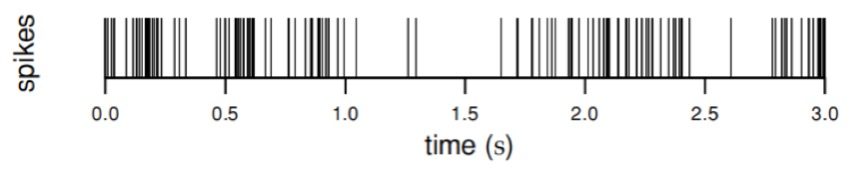
\includegraphics[scale=0.3]{./png/Fig_1_4A.png}
  \end{center}

\begin{alg}
  A simple algorithm of extracting an estimate of the firing rate from a spike train is to divide time into
discrete bins of duration $\Delta t$, count the number of spikes within each bin,
and divide by $\Delta t$.
\end{alg}

\begin{exm}
  \label{fig:1.4B}
  The figure in Example \ref{fig:1.4B} shows the approximate firing rate computed
using this procedure with a bin size of 100 ms. Note that with this procedure, the quantity being computed is 
really the spike-count firing rate over the duration of the bin, and that the firing rate 
r($t$) within a 
given bin is approximated by this spike-count rate. The binning and counting procedure 
illustrated in this figure 
generates an estimate of the firing rate that is a piecewise constant function of time, 
resembling a histogram.
\end{exm}

\begin{center}
  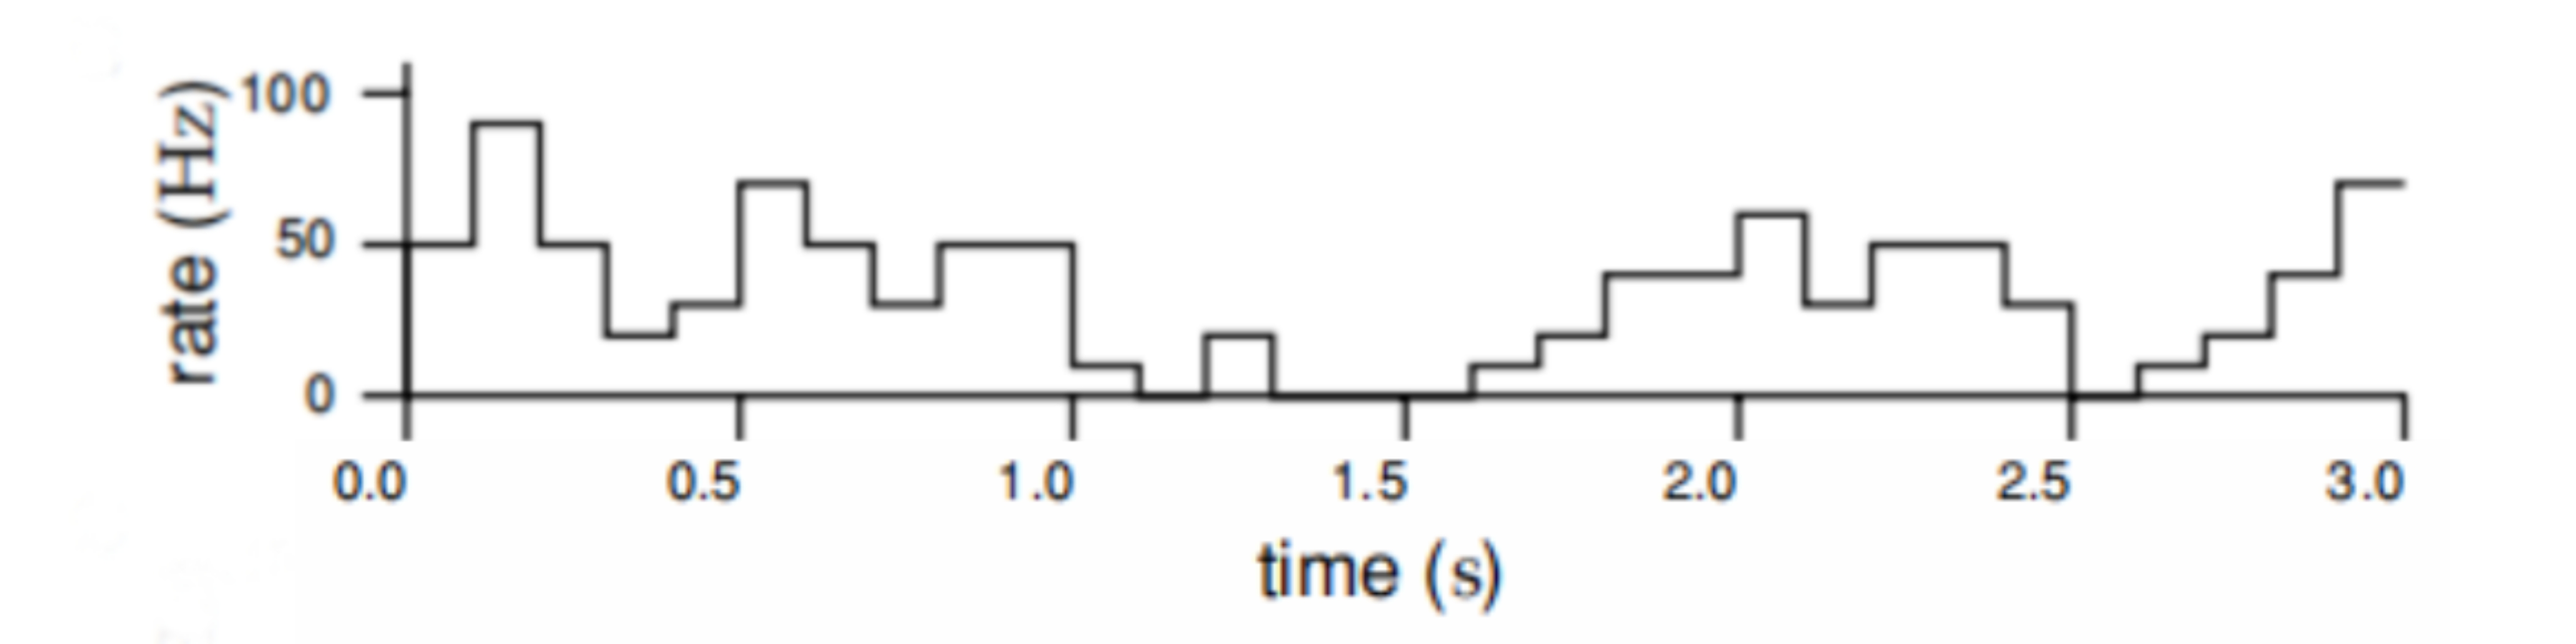
\includegraphics[scale=0.053]{./png/fig_1_4B.png}
\end{center}

\begin{lem}
   Because spike counts can take only integer values, the rates computed by this method will 
   always 
  be integer multiples of $1 / \Delta t$, and thus they take discrete values. Decreasing 
  the value of $\Delta t$
increases temporal resolution by providing an estimate of the firing rate at
more finely spaced intervals of time, but at the expense of decreasing the
resolution for distinguishing different rates.
\end{lem}

\begin{alg}
  One algorithm to avoid quantized
firing rates is to vary the bin size so that a fixed number of spikes appears
in each bin. The firing rate is then approximated as that fixed number of
spikes divided by the variable bin width.
\end{alg}

\begin{rem}
  Counting spikes in preassigned bins produces a firing-rate estimate that
depends not only on the size of the time bins but also on their placement.
\end{rem}

\begin{alg}
To avoid the arbitrariness in the placement of bins, the algorithm is to take
a single bin or window of duration $\Delta t$ and slide it along the spike train,
counting the number of spikes within the window at each location which have a better 
temporal resolution.
\end{alg}

\begin{exm}
  \label{fig:1.4C}
  The jagged curve in the figure of the Example \ref{fig:1.4C} shows the result of sliding a $100$ ms wide
window along the spike train.  The firing rate approximated in 
this way
can be expressed as the sum of a window function over the times $t_i$ for
$i = 1 , 2 ,\dots, n$ when the $n$ spikes in a particular sequence occurred,
\begin{equation}
  \label{equ:1.8}
  \rm{r}_{\text{approx}}(t)=\sum_{i = 1}^{n}\omega(t-t_i), 
\end{equation}
where the window function is

\begin{equation}
  \label{equ:1.9}
  \omega(t)=\left\{
    \begin{aligned}
      1/\Delta t \quad &\text{if} -\Delta t/2\leq t\leq \Delta t/2\\
      0 \quad & \text{otherwise}.
    \end{aligned}
  \right.
\end{equation}
The jagged appearance of the curve is caused 
by the discontinuous shape of the window function used.
\end{exm}

\begin{center}
  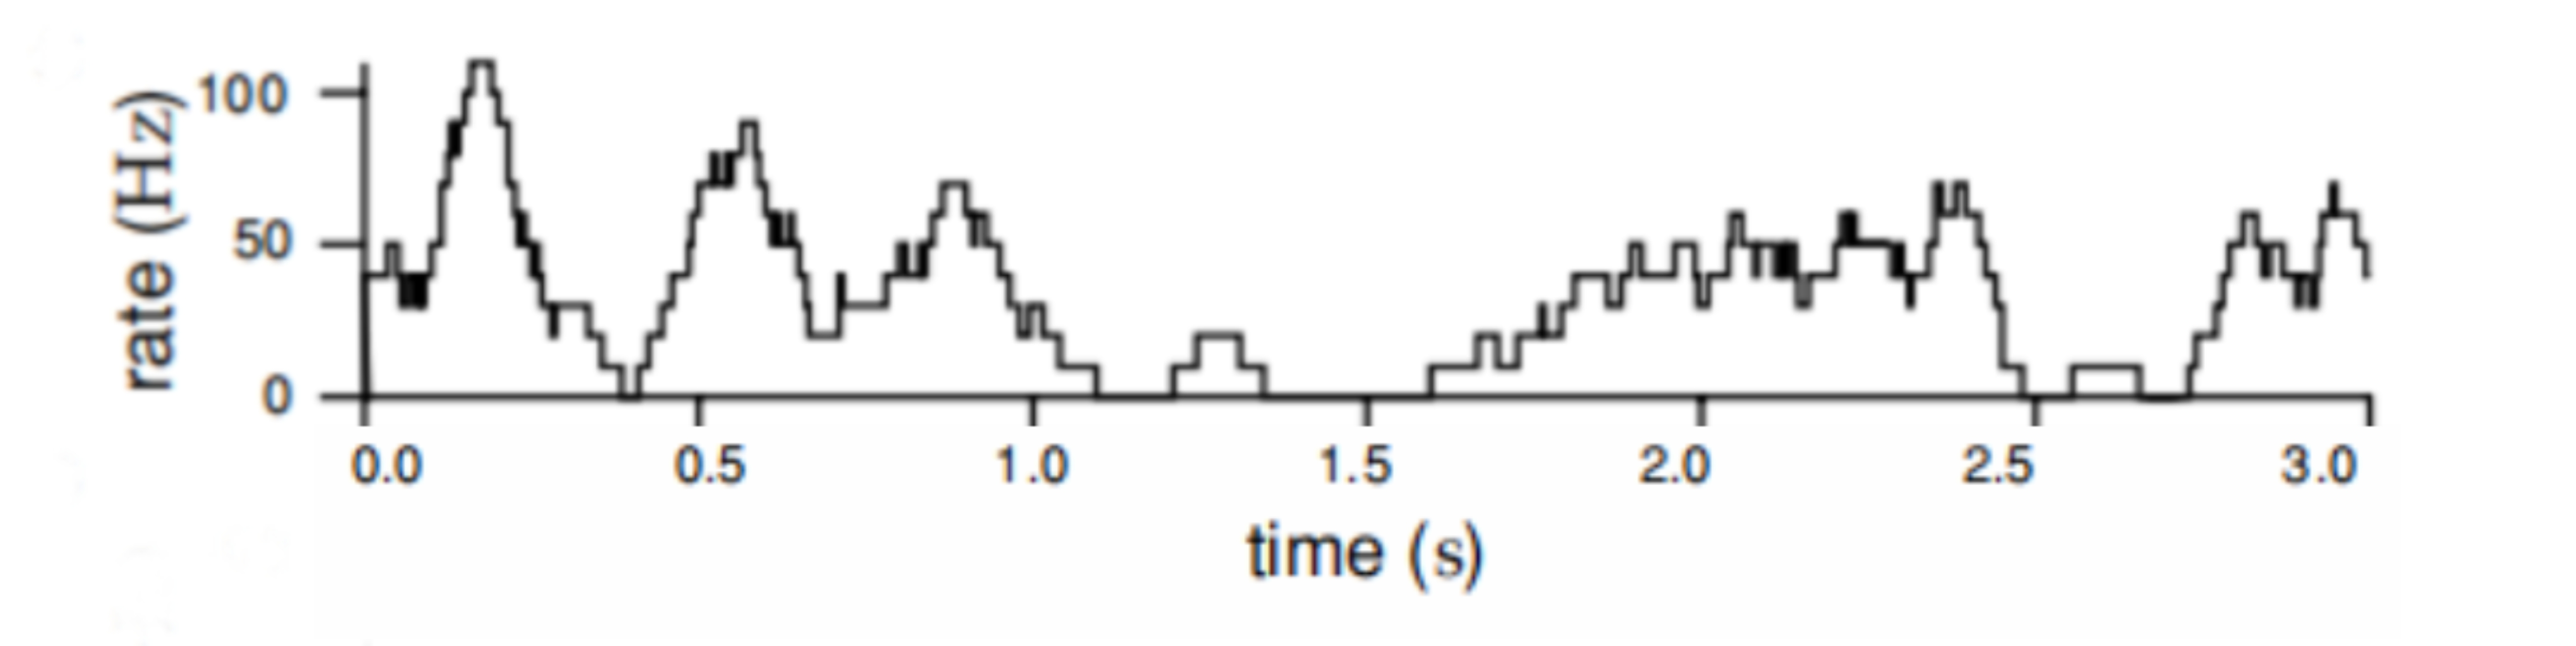
\includegraphics[scale=0.054]{./png/fig_1_4C.png}
\end{center}

\begin{prop}
  The sum in Equation\ref{equ:1.8} can also be written as the integral of the window
function times the neural response function
\begin{equation}
  \label{equ:1.10}
  \rm{r}_{\text{approx}}(t)=\int_{-\infty}^{\infty}\omega(\tau)\rho(t-\tau)d\tau.
\end{equation}
\begin{proof}
  The proof directly follows from Equation \ref{equ:1.2}.
\end{proof}
\end{prop}

\begin{defn}
  The integral in Equation \ref{equ:1.10} is called a \emph{linear filter}, and the window 
  function $\omega$, also called the \emph{filter kernel}, specifies how the neural 
  response function evaluated at time $t-\tau$ contributes to the firing rate approximated 
  at time $t$.
\end{defn}

\begin{exm}
  \label{fig:1.4D}
  Instead of the rectangular window function used in figure in Example \ref{fig:1.4C}, 
  figure in Example \ref{fig:1.4D} use a 
  continuous window function like the Gaussian
  \begin{equation}
    \label{equ:1.11}
    \omega(\tau)=\frac{1}{\sqrt{2\pi}}\sigma_{\omega}\text{exp}\left(-\frac{\tau^2}{2\sigma_{\omega}^2} \right),  
  \end{equation}
   which is used in Equation \ref{equ:1.8} generates 
a firing-rate estimate that is a smooth function of time.
In this case, $\sigma_{\omega}$  controls the temporal resolution of the resulting rate, 
playing a role analogous to $\Delta t$.
\end{exm}

\begin{center}
  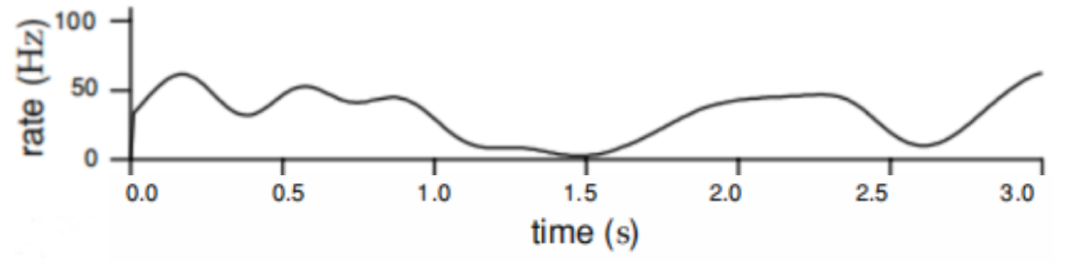
\includegraphics[scale=0.245]{./png/fig_1_4D.png}
\end{center}

\begin{prin}
  A postsynaptic neuron monitoring the spike train of a presynaptic cell has
access only to spikes that have previously occurred.
\end{prin}

\begin{defn}
  A window function or kernel is called \emph{causal} when an approximation
of the firing rate at time $t$ that depends only on spikes fired before $t$ can
be calculated using a window function that vanishes when its argument is negative.

\end{defn}

\begin{defn}
  The \emph{half-wave rectification} $[z]_+$ for any quantity $z$ stands for,
\begin{equation}
  \label{equ:1.13}
  [z]_+ =\left\{
    \begin{aligned}
      z \quad &\text{if} \quad z\geqslant 0\\
      0 \quad & \text{otherwise}.
    \end{aligned}
  \right.
\end{equation}
\end{defn}

\begin{exm}
  \label{fig:1.4E}
  One commonly used window function is the $\alpha$ function
  \begin{equation}
    w(\tau)=[\alpha^2 \tau \text{exp}(-\alpha\tau) ]_+ 
  \end{equation}
  where $1/\alpha$ determines the temporal resolution of the resulting firing-rate
 estimate. The figure below shows the firing rate approximated by such a causal scheme.
\end{exm}

\begin{center}
  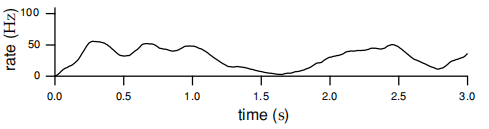
\includegraphics[scale=0.72]{./png/fig_1_4E.png}
\end{center}

\begin{rem}
  Note that the rate computed in Example \ref{fig:1.4E} tends to peak later than the 
  rate computed in Example \ref{fig:1.4D} using a temporally symmetric window function.%%这个地方需要解释一下吗?
\end{rem}

\subsection{Tuning Curve}

\begin{rem}
  Neuronal responses typically depend on many different properties of a
stimulus. In this chapter, we characterize responses of neurons as functions of 
just one of the stimulus attributes to which they may be sensitive. The value of this 
single attribute is denoted by \emph{s}. In chapter \ref{cha:Neural Encoding II}, we consider
more complete stimulus characterizations.
\end{rem}

\begin{defn}
  The \emph{neural response tuning curve} is the average firing rate written 
  as a function of $s$, $\langle r\rangle =f(s)$. The functional form of a tuning 
  curve depends on the parameter $s$ used to describe the stimulus. 
  %The precise choice of parameters used as arguments of tuning curve functions is partially a matter of convention.
\end{defn}

\begin{rem}
  A simple way of characterizing the response of a neuron is to count the
number of action potentials fired during the presentation of a stimulus.
This approach is most appropriate if the parameter $s$ characterizing the
stimulus is held constant over the trial. If we average the number of action potentials 
fired over (in theory, an infinite number of) trials and divide by the trial duration, 
we obtain the average firing rate, $ \langle r\rangle$, defined in Equation \ref{equ:1.7}.
\end{rem}

\begin{ntn}
  Because tuning curves correspond to firing rates, they are measured in units of spikes 
  per second or Hz.
\end{ntn}

\begin{exm}
  \label{fig:1.5}
   We show extracellular recordings of a neuron in the primary visual cortex (V1) of a monkey. While these recordings were being made, a bar of light was moved at different angles across the region of the visual field where the cell responded to light (see figure A). This region is called the receptive  field of the neuron. Note that the number of action potentials fired depends on the angle of orientation of the bar.
\begin{center}
  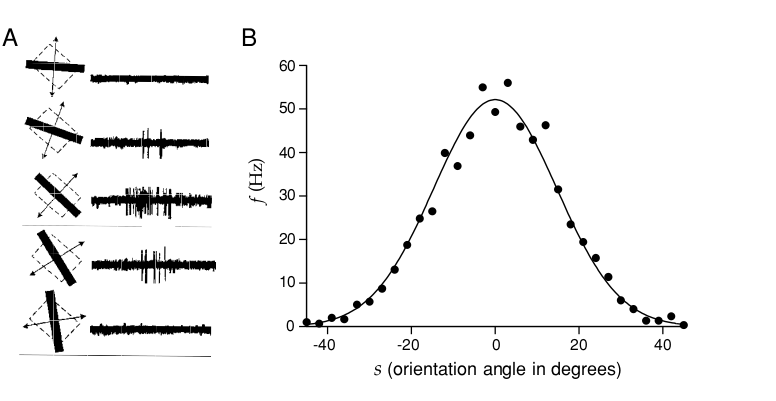
\includegraphics[scale=0.32]{./png/fig_1_5.png}
\end{center}
The dots in figure B indicate the average firing rate depends on the degrees of the orientation angle of the light bar stimulus.
The data have been fitted by a response tuning curve of the form of \emph{Gaussian tuning curve}
\begin{equation}
  \label{equ:1.14}
  f(s)=r_{\text{max}}\text{exp}\left(-\frac{1}{2}\left(\frac{s-s_{\text{max}}}{\sigma_f}\right)^2\right).
\end{equation}
The curve  in figure B is a fit using
the Equation \ref{equ:1.14} with parameters $r_{\text{max}} = 52 . 14 $ Hz, $s_{\text{max}}= 0 ^\circ$,
 and $\sigma_f= 14 . 73 ^\circ $,
where $s$ is the orientation angle of the light bar, $s_{\text{max}}$ is the orientation angle
evoking the maximum average response rate $r_{\text{max}}$ (with $s-s_{\text{max}} $ taken 
to lie in the range between $- 90^\circ $ and $+90^\circ$  ), and $\sigma_f$ determines the 
width of the tuning curve. The neuron responds most vigorously when a stimulus
having $s=s_{\text{max}} $ is presented, so we call $s_{\text{max}}$ the preferred orientation angle
of the neuron.
\end{exm}

\begin{rem}
  Tuning curves can also be measured for neurons in motor areas, in which
case the average firing rate is expressed as a function of one or more parameters describing 
a motor action.
\end{rem}

\begin{exm}
  \label{fig:1.6}
  We show an example of extracellular recordings from a neuron in primary motor cortex 
  in a monkey
  that has been trained to reach in different directions. The stacked traces for
  each direction are rasters showing the results of five different trials. The
  horizontal axis in these traces represents time, and each mark indicates
  an action potential. The firing pattern of the cell, in particular the rate at
  which spikes are generated, is correlated with the direction of arm movement.% and thus 
  encodes information about this aspect of the motor action.
  \begin{center}
    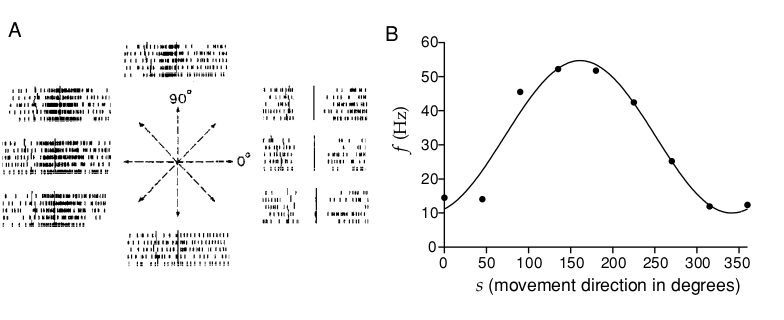
\includegraphics[scale=0.3]{./png/fig_1_6.png}
  \end{center}
  The dots in figure B indicate the average firing rate depends 
  on the degrees of the direction of the arm movement.
  Here the data points have
  been fitted by a tuning curve in the form of a \emph{cosine tuning curve}.
  \begin{equation}
    \label{equ:1.16}
    f(s)=[r_0+\left(r_{\text{max}}-r_0\right)\cos\left(s-s_{\text{max}}\right)]_+,
  \end{equation}
  where $s$ is the reaching angle of the arm, $s_{\text{max}}=161.25^\circ$ is the reaching 
  angle associated with the maximum response $r_{\text{max}}$, and $r_0=32.34$ Hz is an 
  offset or background
  firing rate that shifts the tuning curve up from the zero axis. 
\end{exm}

\begin{exm}
  \label{fig:1.7}
  We show a mode of retinal disparity. The gray lines with arrows show the
location on each retina of an object located nearer than the fixation point F. The
image from the fixation point falls at the fovea in each eye, the small pit where
the black lines meet the retina. The image from a nearer object falls to the left of
the fovea in the left eye and to the right of the fovea in the right eye. For objects
farther away than the fixation point, this would be reversed. The disparity angle $s$
is indicated in the figure.
\begin{center}
  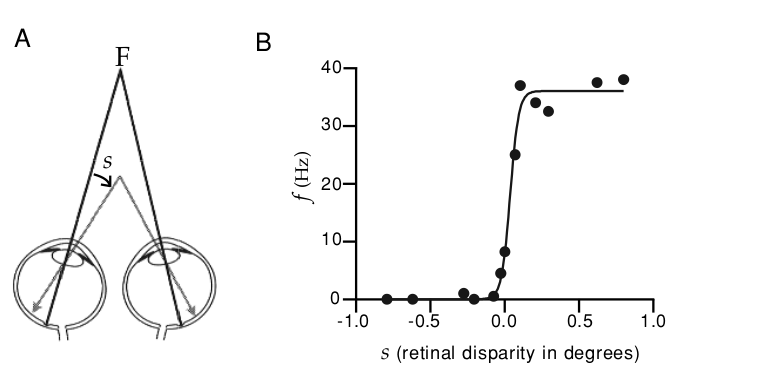
\includegraphics[scale=0.3]{./png/fig_1_7.png}
\end{center}
The dots in figure B indicate average firing rate of a V1 neuron depends on
retinal disparity and illustrates another important type of tuning curve.
Here the data points have been fitted with a tuning curve called
a \emph{logistic function} or \emph{sigmoidal function},
\begin{equation}
  \label{equ:1.17}
  f(s)=\frac{r_{\text{max}}}{1+\exp\left(\left(s_{1/2}-s\right)/\Delta_s\right)}.
\end{equation}
In this case, $s$ is the retinal disparity, the parameter $s_{1/2}$ is the disparity
that produces a firing rate half as big as the maximum value $r_{\text{max}}$ , and $\Delta_s$
controls how quickly the firing rate increases as a function of $s$. If $\Delta_s$ is
negative, the firing rate is a monotonically decreasing function of $s$ rather
than a monotonically increasing function.
\end{exm}

\subsection{Spike-Count Variability}
\begin{rem}
  Tuning curves allow us to predict the average firing rate, but they do not
describe how the spike-count firing rate $r$ varies about its mean value $\langle r\rangle=f(s) $ 
from trial to trial. While the map from stimulus to average
response may be described deterministically, it is likely that single-trial
responses such as spike-count rates can be modeled only in a probabilistic manner.
Generally, $r$ values can be generated from a probability
distribution with mean $f(s)$.
\end{rem}

\begin{defn}
  The trial-to-trial deviation of $r$ from $f ( s )$ is
considered to be noise, and such models are often called \emph{noise models}.
\end{defn}
\begin{defn}
  The standard deviation for the noise distribution either can be independent of 
  $f ( s )$, in which case is called \emph{additive noise}, or it can
depend on $f ( s )$. \emph{Multiplicative noise} corresponds to having the standard
deviation proportional to $f ( s )$.
\end{defn}



%%% Local Variables: 
%%% mode: latex
%%% TeX-master: t
%%% End: 
